\section{Appendix}
In this appendix, we first present additional information about our network architecture and implementation in \cref{sec:supp_network}. We then elaborate on technical details of ego-motion estimation, iterative pose refinement, and scene reconstruction in \cref{sec:supp_method}. Precise definitions of loss functions and evaluation metrics are provided in \cref{sec:supp_loss}. Further analysis of the two datasets, \emph{nuScenes} and \emph{Waymo}, is presented in \cref{sec:supp_dataset}, followed by additional quantitative results including scene flow estimation, instance association, and the TubeNet motion model in \cref{sec:supp_quan}. Finally, we show more qualitative results in \cref{sec:supp_qual}. 

\subsection{Network and implementation}
\label{sec:supp_network}

\paragraph{Network architecture}
The detailed network architecture is depicted in \cref{fig:supp_network}. Our network is a sequential model consisting of (i) per-frame feature extraction used to estimate ego-motion, (ii) multi-frame feature extraction to segment dynamic objects and regress offset vectors towards the associated instance center, and (iii) TubeNet to regress the rigid motions of dynamic objects. The Pillar encoder and the two UNets operate without Batch Normalisation~\cite{ioffe2015batch}, this speeds up training and inference without any loss in performance~\cite{peng2020convolutional}. Our network achieves flexibility w.r.t.\ the number of input frames via global max-pooling along the temporal dimension in the InitConv3D block (\cref{fig:supp_network}).

\paragraph{Implementation details}
We use \texttt{torch\_scatter}\footnote{\url{https://github.com/rusty1s/pytorch_scatter}} to efficiently convert point-wise features to pillar/instance-level global features. To spatially align the backbone features we use \texttt{grid\_sample}, implemented in PyTorch~\cite{NEURIPS2019_9015}. Before clustering, we apply voxel down-sampling implemented in TorchSparse~\cite{tang2022torchsparse} to reduce the point density and improve clustering efficiency. The voxel size is set to 15$\,$cm. Instance labels at full resolution are recovered by indexing points to their associated voxel cell. 

\subsection{Methodology}
\label{sec:supp_method}
\paragraph{Ego-motion estimation}
Given two sets $(\mathbf{P}^1,\mathbf{P}^t)$ of pillar centroid coordinates and associated $L_2$-normalised features $(\mathbf{F}^1_{\ego}, \mathbf{F}^t_{\ego})$, we first compute the cost matrix $\mathbf{M}^t = 2 - 2\langle \mathbf{F}^t_{\ego}, {\mathbf{F}^1_{\ego}}\rangle$ and an Euclidean distance matrix $\mathbf{D}^t_{l,m} = \|\mathbf{p}^t_l - \mathbf{p}^1_m\|_2$ from pillar coordinates. We then pad $\mathbf{M}^t$ with a learnable slack row and column to accommodate outliers, before iteratively alternating between row normalisation and column normalisation\footnote{To improve training stability, row and column normalisations operate in $\log$-space.} for five times to approximate a doubly stochastic permutation matrix $\mathbf{S}^t$ that satisfies
\begin{equation}
    \sum_{l=1}^{N_\ego+1} \mathbf{S}^t_{l, m} =1, \forall m=1, ..., N_\ego,  \quad \sum_{m=1}^{N_\ego+1} \mathbf{S}^t_{l, m} =1, \forall l=1, ..., N_\ego, \quad \mathbf{S}^t_{l,m} \geq 0. 
\end{equation}
Here $\mathbf{S}^t_{l,m}$ represents the probability of $(\mathbf{p}_l^t, \mathbf{p}_m^1)$ being in correspondence. $\mathbf{p}_l^t$ is considered as an outlier and should be ignored during pose estimation if its slack column value $\mathbf{S}^t_{l,-1} \rightarrow 1$.
We further mask $\mathbf{S}^t$ using a support matrix $\mathbf{I}^t$ computed from $\mathbf{D}^t$ as:
\begin{equation}
    \mathbf{I}^t = \left(\mathbf{D}^t < s\right), \quad s = v \cdot \Delta t\;,
\end{equation}
where $v$ is the maximum speed and $\Delta t$ is the interval between two frames. The final corresponding point $\phi(\mathbf{p}_l^t, \mathbf{P}^1)$ of $\mathbf{p}_l^t$ and its weight $w_l^t$ are computed as
\begin{equation}
    \phi(\mathbf{p}_l^t, \mathbf{P}^1) = (\mathbf{I}^t \odot \mathbf{D}^t)_{[l, :-1]} \PC^1, \quad w_l^t = \sum_{m=1}^{N_\ego} (\mathbf{I}^t \odot \mathbf{D}^t)_{l, m}\;,
\end{equation}
with $\odot$ the Hadamard product. \refpaper{eq: ego-motion} is solved with the Kabsch algorithm. For a detailed derivation, please refer to \cite{gojcic2021weakly}. The value of $v$ is dataset-specific, we set it to 30$\,$m/s for the \emph{Waymo}, respectively 10$\,$m/s for \emph{nuScenes}.

\paragraph{Iterative refinement of TubeNet estimates}
To improve the estimation of the transformation parameters for dynamic objects, we unroll TubeNet for two iterations, as often done in point cloud registration~\cite{yew2020rpm,gojcic2020multiview}. Specifically, for a dynamic object $\PC_k$, we first estimate the initial rigid transformation $\mathbf{T}_k^{0, t}$ of the $t^\text{th}$ frame $\mathbf{X}_k^t$ following \refpaper{eq:tubenet}. We then obtain the transformed points $\mathbf{X}_k^{t'} = \mathbf{T}_k^{0, t} \circ \mathbf{X}_k^t$. Next, we update the positional feature $\agfeature_\pos^{t'} = \PN(\PC_k^{t'})$ and regress the residual transformation matrix $\mathbf{T}_k^{t, 1}$ again, according to \refpaper{eq:tubenet}. The final transformation is $\mathbf{T}_k^{t, 1}\cdot\mathbf{T}_k^{t, 0}$. For better stability during training, the gradients between the two iterations are detached. We assign higher weight to the latter iteration to improve accuracy. The overall loss $\loss_\obj^\lcircle{losspurple}$ is:
\begin{equation}
    \loss_\obj^\lcircle{losspurple} = 0.7\cdot \loss_\obj^{\lcircle{losspurple},0} +  \loss_\obj^{\lcircle{losspurple},1}
\end{equation}

\paragraph{Scene reconstruction}
To show the benefits of our method for downstream tasks, we use the points accumulated with different methods as a basis for 3D surface reconstruction, see \cref{fig:supp_nuscene,fig:supp_waymo}. Specifically, we use the accumulated points as input to the Poisson reconstruction~\cite{kazhdan2006poisson}, implemented in Open3D~\cite{Zhou2018}. To estimate point cloud normals, the neighborhood radius is set to 0.5$\,$m and the maximum number of neighbors is set to 128. The depth for the Poisson method is set to 10, and the reconstructed meshes are filtered by removing vertices with densities below the 15$^\text{th}$ percentile. 

\subsection{Loss functions and evaluation metrics}
\label{sec:supp_loss}
\paragraph{Weighted BCE loss}
To compensate for class imbalance, we use a weighted BCE and compute the weights of each class on the fly. Specifically, for a mini-batch with $N_{\text{pos}}$ positive and $N_{\text{neg}}$ negative samples, the associated weights $w_{\text{pos}}$ and $w_{\text{neg}}$ are computed as:
\begin{equation}
    w_{\text{pos}} = \min(\sqrt{\frac{N_{\text{pos}} + N_{\text{neg}}}{N_{\text{pos}}}}, w_{\text{max}}) \qquad 
    w_{\text{neg}} = \min(\sqrt{\frac{N_{\text{pos}} + N_{\text{neg}}}{N_{\text{neg}}}}, w_{\text{max}})\;,
\end{equation}
where $w_{\text{max}}$ is the maximum weight of a class.\footnote{We find that in some extreme cases, there are very few ($<10$) positive samples and way more negative samples. We thus bound $w_{\text{max}}$ at 50 to ensure stability.} The final weighted BCE loss $\mathcal{L}_{\mathrm{bce}}(\mathbf{x}, \overline{\mathbf{x}})$ is 
\begin{equation}
\mathcal{L}_{\mathrm{bce}}(\mathbf{x}, \overline{\mathbf{x}}) \!= \frac{1}{|\mathbf{x}|} \sum_{i=1}^{|\mathbf{x}|} w_i (\overline{\mathbf{x}}_i \log(\mathbf{x}_i) + (1 - \overline{\mathbf{x}}_i) \log (1 - \mathbf{x}_i))\;,
\end{equation}
with $\mathbf{x}$ and $\overline{\mathbf{x}}$ are predicted and ground truth labels, and $w_i$ the weight of the $i^\text{th}$ sample, computed as
\begin{equation}
    w_i =      
    \begin{cases}
      w_{\text{pos.}}, & \text{if } \overline{\mathbf{x}}_i = 1  \\
      w_{\text{neg.}}, & \text{otherwise}
    \end{cases}\;.
\end{equation}

\paragraph{Lov\'{a}sz-Softmax loss}
The Jaccard index (ratio of Intersection over Union) is commonly used to measure segmentation quality. In the binary classification setting, we can set the ground truth labels as $\overline{\mathbf{x}}_i \in \{-1,1\}$, then the Jaccard index of the foreground class $J_1$ is computed as
\begin{equation}
    J_1(\overline{\mathbf{x}}, \mathbf{x}) = \frac{|\{\overline{\mathbf{x}} = 1\} \cap \{\mathrm{sign}(\mathbf{x}) = 1\}|}{|\{\overline{\mathbf{x}} = 1\} \cup \{\mathrm{sign}(\mathbf{x}) = 1\}|}\;, \quad J_1(\overline{\mathbf{x}}, \mathbf{x}) \in [0,1]\;,
\end{equation}
with $\mathbf{x}$ the prediction and $\mathrm{sign}()$ the sign function. The corresponding loss $\Delta_{J_1}(\overline{\mathbf{x}}, \mathbf{x})$ to minimise the empirical risk is
\begin{equation}
    \Delta_{J_1}(\overline{\mathbf{x}}, \mathbf{x}) = 1 - J_1(\overline{\mathbf{x}}, \mathbf{x})\;.
\end{equation}
However, this is not differentiable and cannot be directly employed as a loss function. The authors of~\cite{berman2018lovasz} have proposed to optimise it using a Lov\'{a}sz extension. The Lov\'{a}sz extension $\dddot{\Delta}$ of a set function $\Delta$ is defined as:
\begin{equation}
    \dddot{\Delta} (\mathbf{m}) = \sum_{i=1}^{p} \mathbf{m}_i \, g_i(\mathbf{m})\;,
\end{equation}
with 
\begin{equation}
g_i(\mathbf{m}) =
\Delta(\{\pi_1, \ldots, \pi_i\})- \Delta(\{\pi_1, \ldots, \pi_{i-1}\}),
\end{equation}
where $\mathbf{\pi}$ denotes a permutation that places the components of $\mathbf{m}$ in decreasing order. Considering $\mathbf{m}_i = \max(1 - \mathbf{x}_i \overline{\mathbf{x}}_i, 0)$, the Lov\'{a}sz-Softmax loss $\mathcal{L}_{ls}(\overline{\mathbf{x}}, \mathbf{x})$ is defined as 
\begin{equation}
    \mathcal{L}_{ls}(\overline{\mathbf{x}}, \mathbf{x}) = \dddot{\Delta_{J_1}}(\mathbf{m}).
\end{equation}


\paragraph{Inlier loss}
Previous works~\cite{yew2020rpm,gojcic2021weakly} have observed that the entropy-regularized optimal transport~\cite{cuturi2013sinkhorn} has a tendency to label most points as outliers. To alleviate this issue, we follow~\cite{yew2020rpm,gojcic2021weakly} and use an inlier loss $\mathcal{L}_{\text{inlier}}$ on the matching matrix $\mathbf{D}^t$, designed to encourage inliers. The inlier loss is defined as
\begin{equation}
    \mathcal{L}_{\text{inlier}}^t = \frac{1}{2N_{\ego}} (2N_{\ego} - \sum_{l=1}^{N_\ego} \sum_{m=1}^{N_\ego} \mathbf{D}_{l,m}^t)\;.
\end{equation}


\paragraph{Instance association metrics}
To quantitatively measure the spatio-temporal instance association quality, we report weighted coverage (\textit{WCov}) as well as recall and precision at a certain threshold. Given the ground truth clusters $\mathcal{G}$ and the estimated clusters $\mathcal{O}$, recall measures the ratio of clusters in $\mathcal{G}$ that have an overlap above some threshold with a cluster in $\mathcal{O}$, while precision does the same in the opposite direction. Weighted coverage $WCov (\mathcal{G},\mathcal{O})$ is computed as
\begin{equation}
    WCov(\mathcal{G}, \mathcal{O}) = \sum_{i=1}^{|\mathcal{G}|} \frac{1}{|\mathcal{G}|} w_i \max_j \mathrm{IoU} (r_i^G, r_j^0), \qquad  w_i = \frac{|r_i^G|}{\sum_k |r_k^G|}\;,
\end{equation}
where $r_i^G$ and $r_j^O$ are clusters from $\mathcal{G}$ and $\mathcal{O}$, and $\mathrm{IoU}(r_i^G, r_j^O)$ denotes the overlap between two clusters. 

\paragraph{ECDF}
The Empirical Cumulative Distribution Function (ECDF) measures the distribution of a set of values:
\begin{equation}
\begin{aligned}
\text{ECDF} (x) = \frac{\big|\{o_i < x\}\big|}{\big|O\big|}\;,
\end{aligned}
\end{equation}
where $O = \{o_i\}$ is a set of samples and $x \in [\min\{O\}, \max\{O\}]$.

\subsection{Dataset analysis}
\label{sec:supp_dataset}
\begin{figure}[t!]
     \centering
        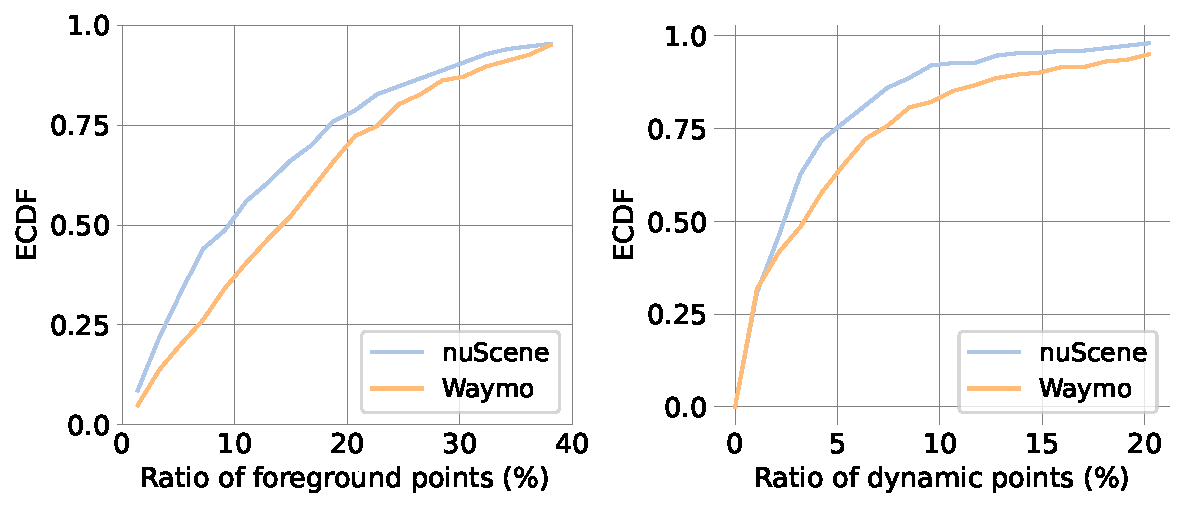
\includegraphics[width=1.0\columnwidth]{figs/figure/dataset_stats.pdf}
       \caption{\textit{ECDF} curve of points lying on foreground objects and on dynamic objects, for both the \emph{Waymo} and \emph{nuScenes} datasets.}
   \label{fig:dataset_ecdf}
\end{figure}
\begin{figure}[t!]
     \centering
        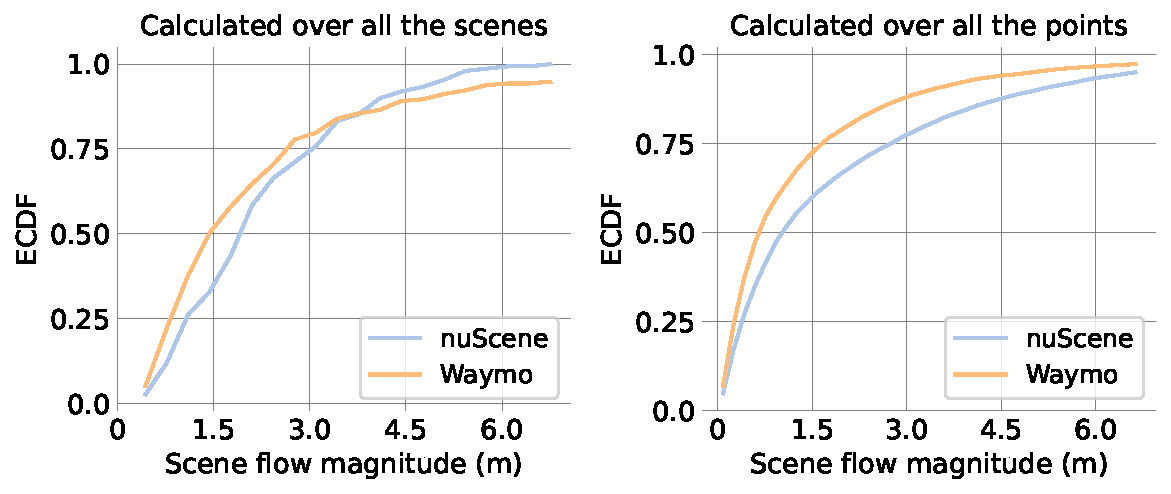
\includegraphics[width=1.0\columnwidth]{figs/figure/motion.pdf}
       \caption{Scene flow magnitudes of dynamic objects in the \emph{Waymo} and \emph{nuScenes} datasets.}
   \label{fig:motion_ecdf}
\end{figure}
In total, we have 150, respectiverly 202 scenes as held-out test sets in \emph{nuScenes} and \emph{Waymo}. The \textit{ECDF} curve of points belonging to foreground and dynamic objects are shown in \cref{fig:dataset_ecdf}. As can be seen, the ratios of foreground and dynamic points span a large range (40\% and 20\%). Recalling that the scene flow estimation performance of the dynamic parts falls far behind that of the static parts (\refpaper{tab:sf_main}), this large range of ratios of dynamic objects hints at different difficulties across the scenes. The median fractions of foreground points are 16.2\%/9.4\% in \emph{Waymo}/\emph{nuScenes}, the median fractions of points on moving objects are 3.5\%/2.4\%. In other words, roughly 75\% of all foreground objects are static. This motivates
our strategy to start with motion segmentation, so as to make explicit the large static component (including many objects that could move) whose scene flow is identical to the ego-motion.

In \cref{fig:motion_ecdf}, we show the \textit{ECDF} curve of scene flow magnitudes ($L_2$-norm of scene flow vectors) for the dynamic portions of the two datasets. The motions span a large range, but 75\% of the flow vectors are of moderate magnitude \textless3$\,$m. \emph{nuScenes} has slightly larger overall flow magnitudes than \emph{Waymo}, but \emph{Waymo} contains more instances of large motions (\cref{fig:motion_ecdf}~(left)).

\subsection{Additional results}
\label{sec:supp_quan}
\paragraph{Results averaged over scenes}
\begin{table}[t]
    \setlength{\tabcolsep}{6pt}
    \renewcommand{\arraystretch}{1.2}
	\centering
	\resizebox{\columnwidth}{!}{
    \begin{tabular}{clcccc|ccccc}
    \toprule
    & & \multicolumn{4}{c|}{Static part} & \multicolumn{4}{c}{Dynamic foreground}  \\
    Dataset  & Method  & EPE avg.$\downarrow$ & AccR$\uparrow$  & AccS$\uparrow$ & ROutlier$\downarrow$ & EPE avg. $\downarrow$ & AccR$\uparrow$   & AccS$\uparrow$   & ROutliers $\downarrow$ \\
    \midrule
    \multirow{5}{*}{\emph{Waymo}} & PPWC-Net~\cite{wu2019pointpwc}  &  0.475 $\pm$ 0.543 & 35.0 & 14.2 & 13.5 & 0.658 $\pm$ 0.696 & 27.1 & 7.9 & 22.9\\
                              & FLOT~\cite{puy2020flot} &   0.381 $\pm$ 0.516 & 68.8 & 51.8 & 13.0 & 0.772 $\pm$ 0.711 & 30.1 & 11.2 & 31.9\\
                              & WsRSF~\cite{gojcic2021weakly} & 1.415 $\pm$ 1.352 & 34.6 & 23.0 & 56.9 & 1.764 $\pm$ 1.744 & 21.0 & 8.6 & 61.6\\
                              & NSFPrior~\cite{li2021neural} & 0.159 $\pm$ 0.231 & 87.1 & 73.5 & 4.3 & 0.355 $\pm$ 0.456 & 63.7 & 41.3 & 14.3 \\
                              & Ours & \textbf{0.088} $\pm$ 0.237 & \textbf{91.6} & \textbf{81.9} & \textbf{2.3} & \textbf{0.169} $\pm$ 0.259 & \textbf{76.8} & \textbf{52.9} & \textbf{5.3}\\
    \midrule
    \multirow{5}{*}{\emph{nuScenes}} & PPWC-Net~\cite{wu2019pointpwc} & 0.488 $\pm$ 0.402 & 34.2 & 12.7 & 17.5 & 0.784 $\pm$ 0.547 & 22.8 & 6.9 & 35.0 \\
                                  & FLOT~\cite{puy2020flot} & 0.597 $\pm$ 0.582 & 53.3 & 35.1 & 26.6 & 1.156 $\pm$ 0.714 & 13.2 & 3.7 & 56.5\\
                                  & WsRSF~\cite{gojcic2021weakly} & 0.658 $\pm$ 0.483 & 47.5 & 31.1 & 31.5 & 0.925 $\pm$ 0.627 & 29.8 & 15.0 & 42.2\\
                                  & NSFPrior~\cite{li2021neural} & 0.501 $\pm$ 0.344 & 57.8 & 37.7 & 21.3 & 0.743 $\pm$ 0.537 & 39.1 & 19.9 & 31.1 \\
                                   & Ours & \textbf{0.226} $\pm$ 0.206 & \textbf{72.3} & \textbf{46.7} & \textbf{7.4} & \textbf{0.394} $\pm$ 0.26 & \textbf{47.8} & \textbf{22.7} & \textbf{17.3}\\
    \bottomrule
    \end{tabular}
    }
	\caption{Scene flow estimation results on \emph{Waymo} and \emph{nuScenes} datasets. Numbers are averaged over all test scenes.}
	\label{tab:sf_supp}
\end{table}\textbf{}


% \begin{table}[t]
%     \setlength{\tabcolsep}{6pt}
%     \renewcommand{\arraystretch}{1.2}
% 	\centering
%     \begin{tabularx}{\textwidth}{YlYYYY|YYYYY}
%     \toprule
%     & & \multicolumn{4}{c|}{Static part} & \multicolumn{4}{c}{Dynamic foreground}  \\
%     Dataset  & Method  & EPE avg.$\downarrow$ & AccR$\uparrow$  & AccS$\uparrow$ & ROutlier$\downarrow$ & EPE avg. $\downarrow$ & AccR$\uparrow$   & AccS$\uparrow$   & ROutliers $\downarrow$ \\
%     \midrule
%     \multirow{5}{*}{\emph{Waymo}} & PPWC-Net~\cite{wu2019pointpwc}  &  0.475 $\pm$ 0.543 & 35.0 & 14.2 & 13.5 & 0.658 $\pm$ 0.696 & 27.1 & 7.9 & 22.9\\
%                               & FLOT~\cite{puy2020flot} &   0.381 $\pm$ 0.516 & 68.8 & 51.8 & 13.0 & 0.772 $\pm$ 0.711 & 30.1 & 11.2 & 31.9\\
%                               & WsRSF~\cite{gojcic2021weakly} & 1.415 $\pm$ 1.352 & 34.6 & 23.0 & 56.9 & 1.764 $\pm$ 1.744 & 21.0 & 8.6 & 61.6\\
%                               & NSFPrior~\cite{li2021neural} & 0.159 $\pm$ 0.231 & 87.1 & 73.5 & 4.3 & 0.355 $\pm$ 0.456 & 63.7 & 41.3 & 14.3 \\
%                               & Ours & \textbf{0.088} $\pm$ 0.237 & \textbf{91.6} & \textbf{81.9} & \textbf{2.3} & \textbf{0.169} $\pm$ 0.259 & \textbf{76.8} & \textbf{52.9} & \textbf{5.3}\\
%     \midrule
%     \multirow{5}{*}{\emph{nuScenes}} & PPWC-Net~\cite{wu2019pointpwc} & 0.488 $\pm$ 0.402 & 34.2 & 12.7 & 17.5 & 0.784 $\pm$ 0.547 & 22.8 & 6.9 & 35.0 \\
%                                   & FLOT~\cite{puy2020flot} & 0.597 $\pm$ 0.582 & 53.3 & 35.1 & 26.6 & 1.156 $\pm$ 0.714 & 13.2 & 3.7 & 56.5\\
%                                   & WsRSF~\cite{gojcic2021weakly} & 0.658 $\pm$ 0.483 & 47.5 & 31.1 & 31.5 & 0.925 $\pm$ 0.627 & 29.8 & 15.0 & 42.2\\
%                                   & NSFPrior~\cite{li2021neural} & 0.501 $\pm$ 0.344 & 57.8 & 37.7 & 21.3 & 0.743 $\pm$ 0.537 & 39.1 & 19.9 & 31.1 \\
%                                    & Ours & \textbf{0.226} $\pm$ 0.206 & \textbf{72.3} & \textbf{46.7} & \textbf{7.4} & \textbf{0.394} $\pm$ 0.26 & \textbf{47.8} & \textbf{22.7} & \textbf{17.3}\\
%     \bottomrule
%     \end{tabularx}
% 	\caption{Scene flow estimation results on \emph{Waymo} and \emph{nuScenes} datasets. Numbers are averaged over all test scenes.}
% 	\label{tab:sf_supp}
% \end{table}\textbf{}
In \refpaper{tab:sf_main} we report evaluation metrics calculated over all the points in the test set. However, this does not fully reveal the difficulties encountered in different scenes. Here, we first calculate evaluation metrics per scene, then report the average over scenes in \cref{tab:sf_supp}. For \textit{EPE avg.}, we additionally report the standard deviations. We can see that for both static and dynamic parts, all methods have large standard deviations, which indicates varying difficulty of the scenes, as well as gross errors from challenging samples. Our model still achieves the smallest flow errors and standard deviations under this evaluation setting, for both datasets . 


\paragraph{Spatio-temporal instance association}
\begin{figure}[t]
     \centering
        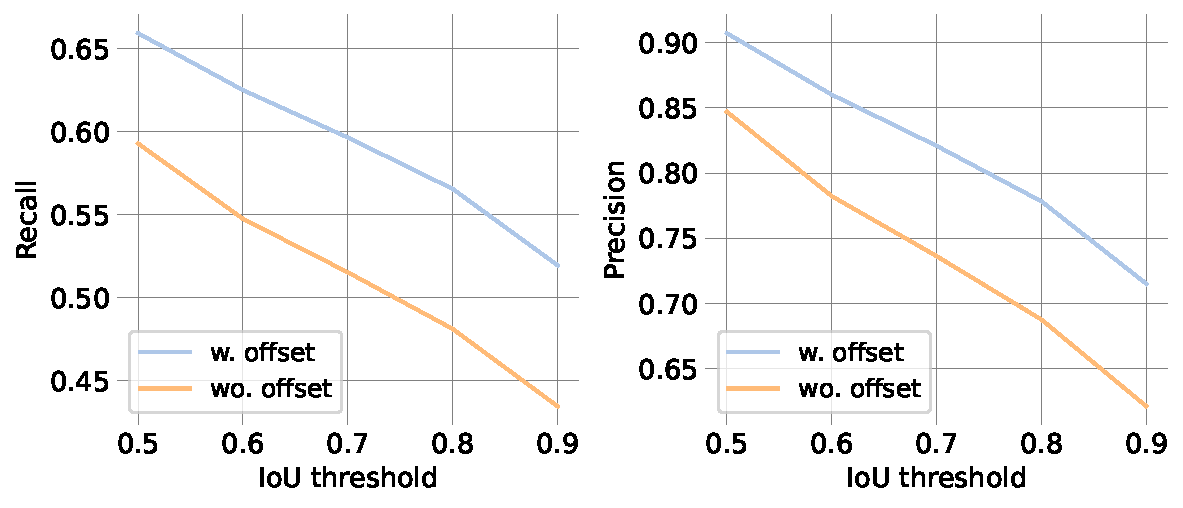
\includegraphics[width=0.8\columnwidth]{figs/figure/association.pdf}
       \caption{Spatio-temporal instance association performance on \emph{Waymo} with and without offset prediction.}
   \label{fig:supp_association}
\end{figure}
We plot instance association metrics at different thresholds in \cref{fig:supp_association}. As can be seen, offset prediction improves association recall and precision by \textgreater5\%, across a range of thresholds. Such improvement becomes more significant as one increases the \textit{IoU} threshold, reaching $\approx$10\% at $IoU=0.9$. We conclude that offset prediction is important to retain high-quality spatio-temporal instances, which can subsequently improve the accuracy of motion modelling for the dynamic parts (\textit{AccS} increases by 9.2\%  in \refpaper{tab:ablations}).


\begin{table}[t]
    \setlength{\tabcolsep}{6pt}
    \renewcommand{\arraystretch}{1.2}
	\centering
    \begin{tabular}{clcccccc}
    \toprule
   &  & EPE avg.$\downarrow$ & EPE med.$\downarrow$ & AccS$\uparrow$ & AccR$\uparrow$ & ROutliers$\downarrow$   \\
   \midrule
    \multirow{3}{*}{\emph{Waymo}} & center & 0.265 & 0.095 & 36.9 & 62.9 & 9.9\\ 
    & center + ICP  & 0.212 & 0.047 & 61.2 & 80.0 & 7.7 \\
    & Ours   & 0.197 & 0.062 & 53.3 & 77.5 & 5.9 \\
    & Ours + ICP   & \textbf{0.173} & \textbf{0.043} & \textbf{69.1} & \textbf{86.9} & \textbf{5.1}\\
    \midrule
    \multirow{3}{*}{\emph{nuScenes}} & center & 0.553 & 0.258 & 13.5 & 32.7 & 28.2     \\ 
    & center + ICP   & 0.525 & 0.179 & 23.8 & 43.7 & 25.5\\
    & Ours   & 0.301 & 0.146 & 26.6 & 53.4 & \textbf{12.1}    \\
    & Ours + ICP   & \textbf{0.301} & \textbf{0.135} & \textbf{32.7} & \textbf{56.7} & 13.7 \\
    \bottomrule
    \end{tabular}
	\caption{Comparison to centroid-based motion estimation baseline.}
	\label{tab:tubenet_comparison}
\end{table}
\paragraph{Dynamic object motion modelling}
We additionally compare the proposed TubeNet to two baseline methods. We naively align each frame $\PC_k^t$ $(t>1)$ of an instance $\PC_k$ to frame $\PC_k^0$ by %
translating the centroids, and term this method \textit{center}. For \textit{center+ICP} we refine the simple translational alignment by a subsequent ICP. The detailed comparison is shown in \cref{tab:tubenet_comparison}. Our learned TubeNet achieves the best performance on both datasets. The improvement is larger on the challenging \emph{nuScenes} data, where the point clouds are sparser and less complete, so centroids computed from partial observations are not an accurate proxy for the object location. Our learned TubeNet can implicitly exploit prior knowledge about object shape and surface-level correspondence, leading to more robust and accurate motion modelling. 

\subsection{Qualitative results}
\label{sec:supp_qual}
We show additional qualitative results in \cref{fig:supp_waymo} and \cref{fig:supp_nuscene}. Benefiting from the explicit \textit{multi-body} assumption, our model achieves accurate scene flow estimation of both static parts (\cref{fig:supp_waymo} (1) and \cref{fig:supp_nuscene} (2)) and dynamic parts (\cref{fig:supp_waymo} (3) and \cref{fig:supp_nuscene}(1)). Errors in the automatically generated pseudo-ground truth are shown in \cref{fig:supp_nuscene}(3), in this case our model achieves more accurate flow estimation and reconstruction.  

\begin{figure}[t]
     \centering
        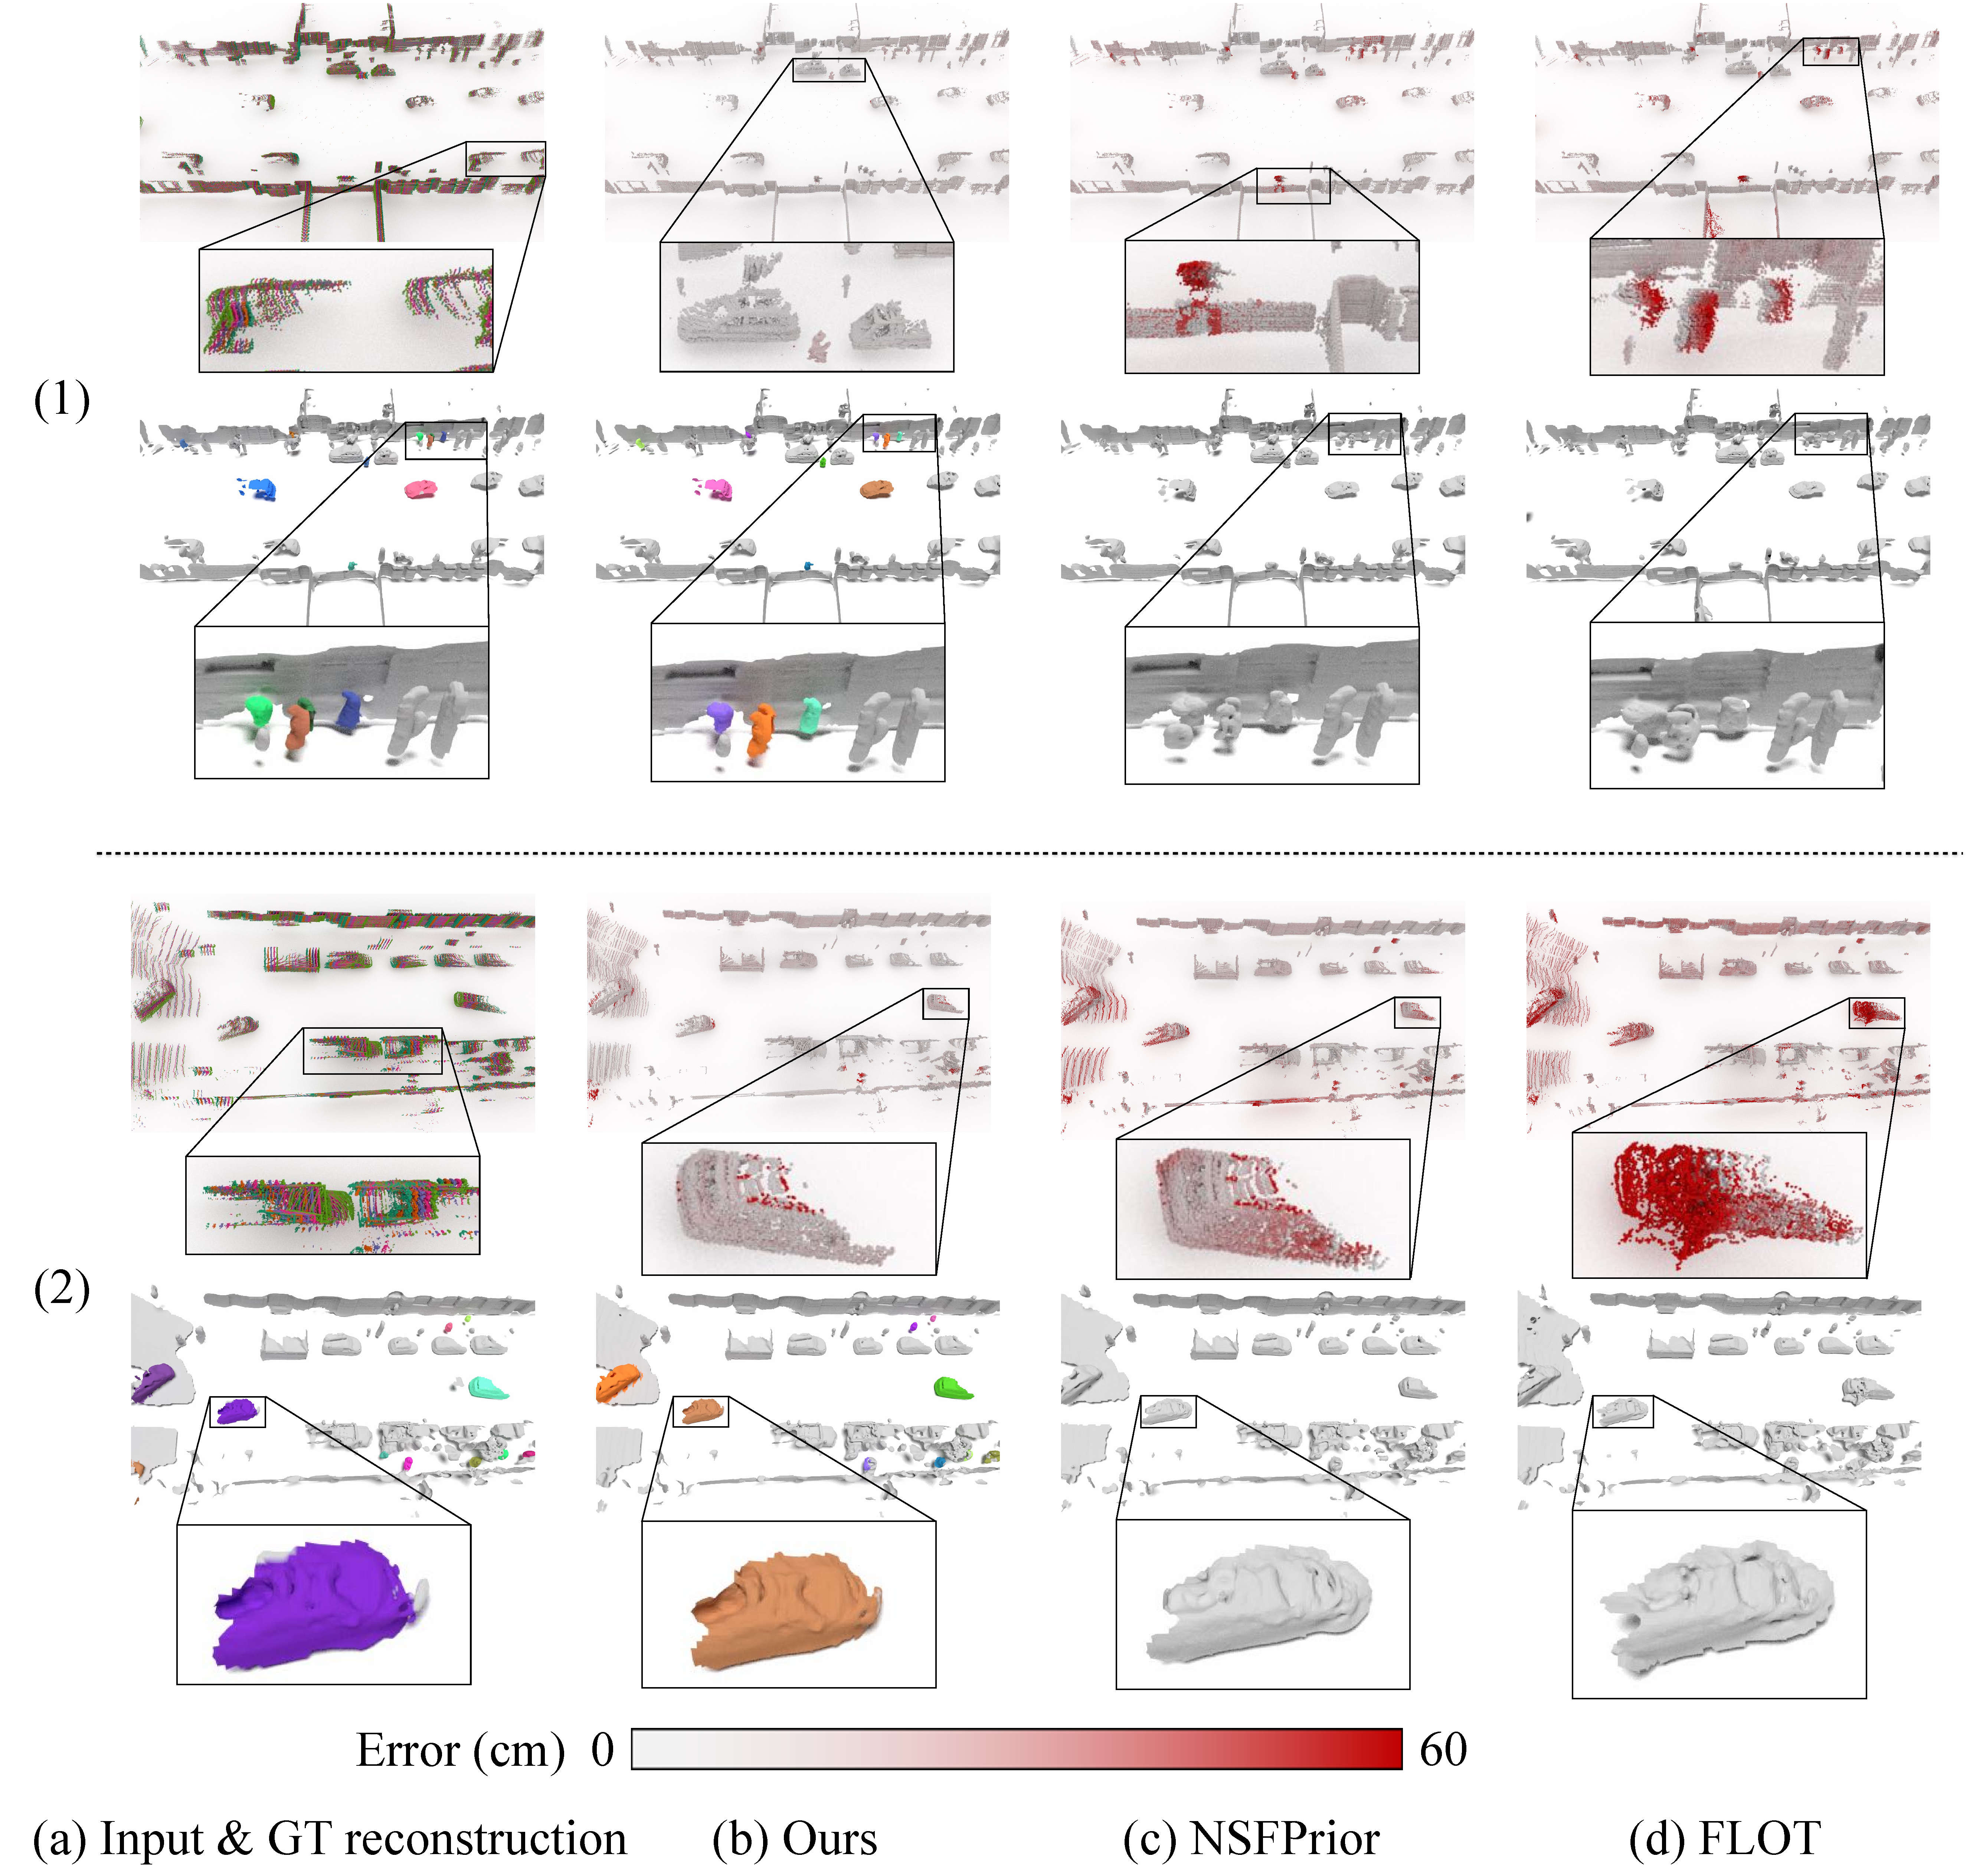
\includegraphics[width=\columnwidth]{figs/figure/supp_waymo.pdf}
       \caption{Qualitative results showing scene flow estimation (top) and surface reconstruction (bottom) for three example scenes from the \emph{Waymo} dataset.}
   \label{fig:supp_waymo}
\end{figure}
\begin{figure}[t]
     \centering
        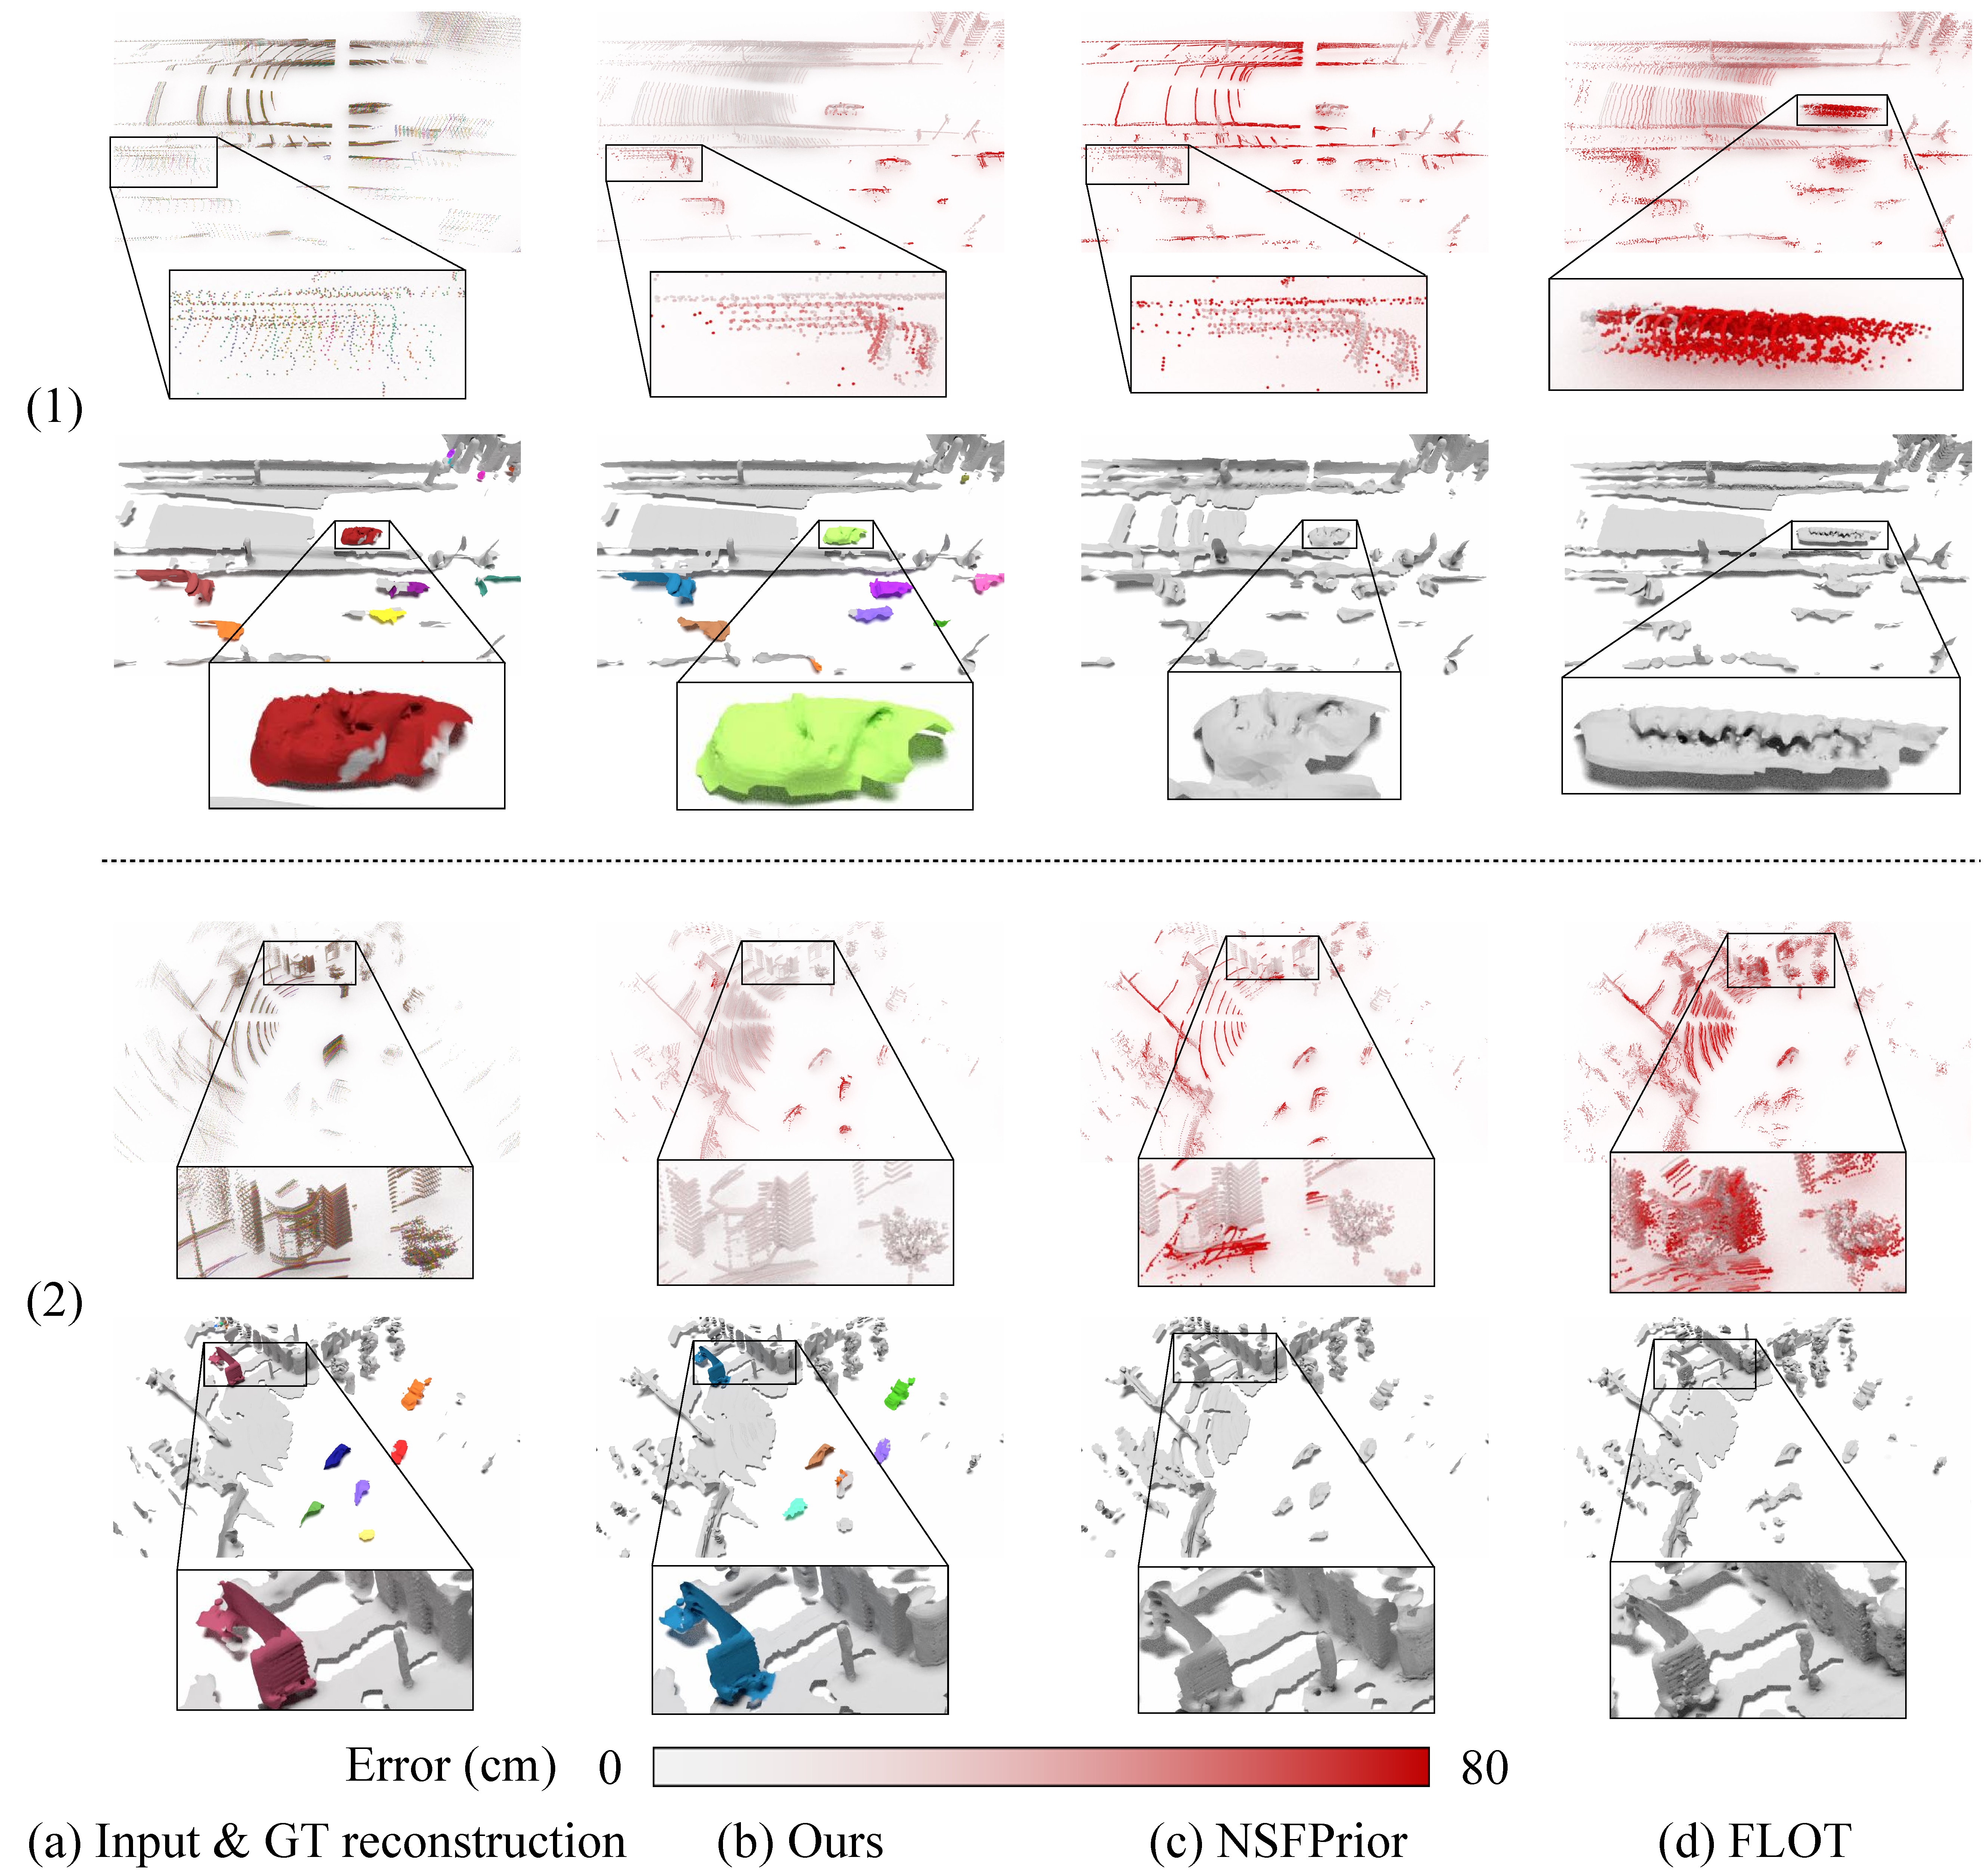
\includegraphics[width=\columnwidth]{figs/figure/supp_nuscene.pdf}
       \caption{Qualitative results showing scene flow estimation (top) and surface reconstruction (bottom) for three example scenes from the \emph{nuScenes} dataset.}
   \label{fig:supp_nuscene}
\end{figure}
\begin{figure}[t]
     \centering
        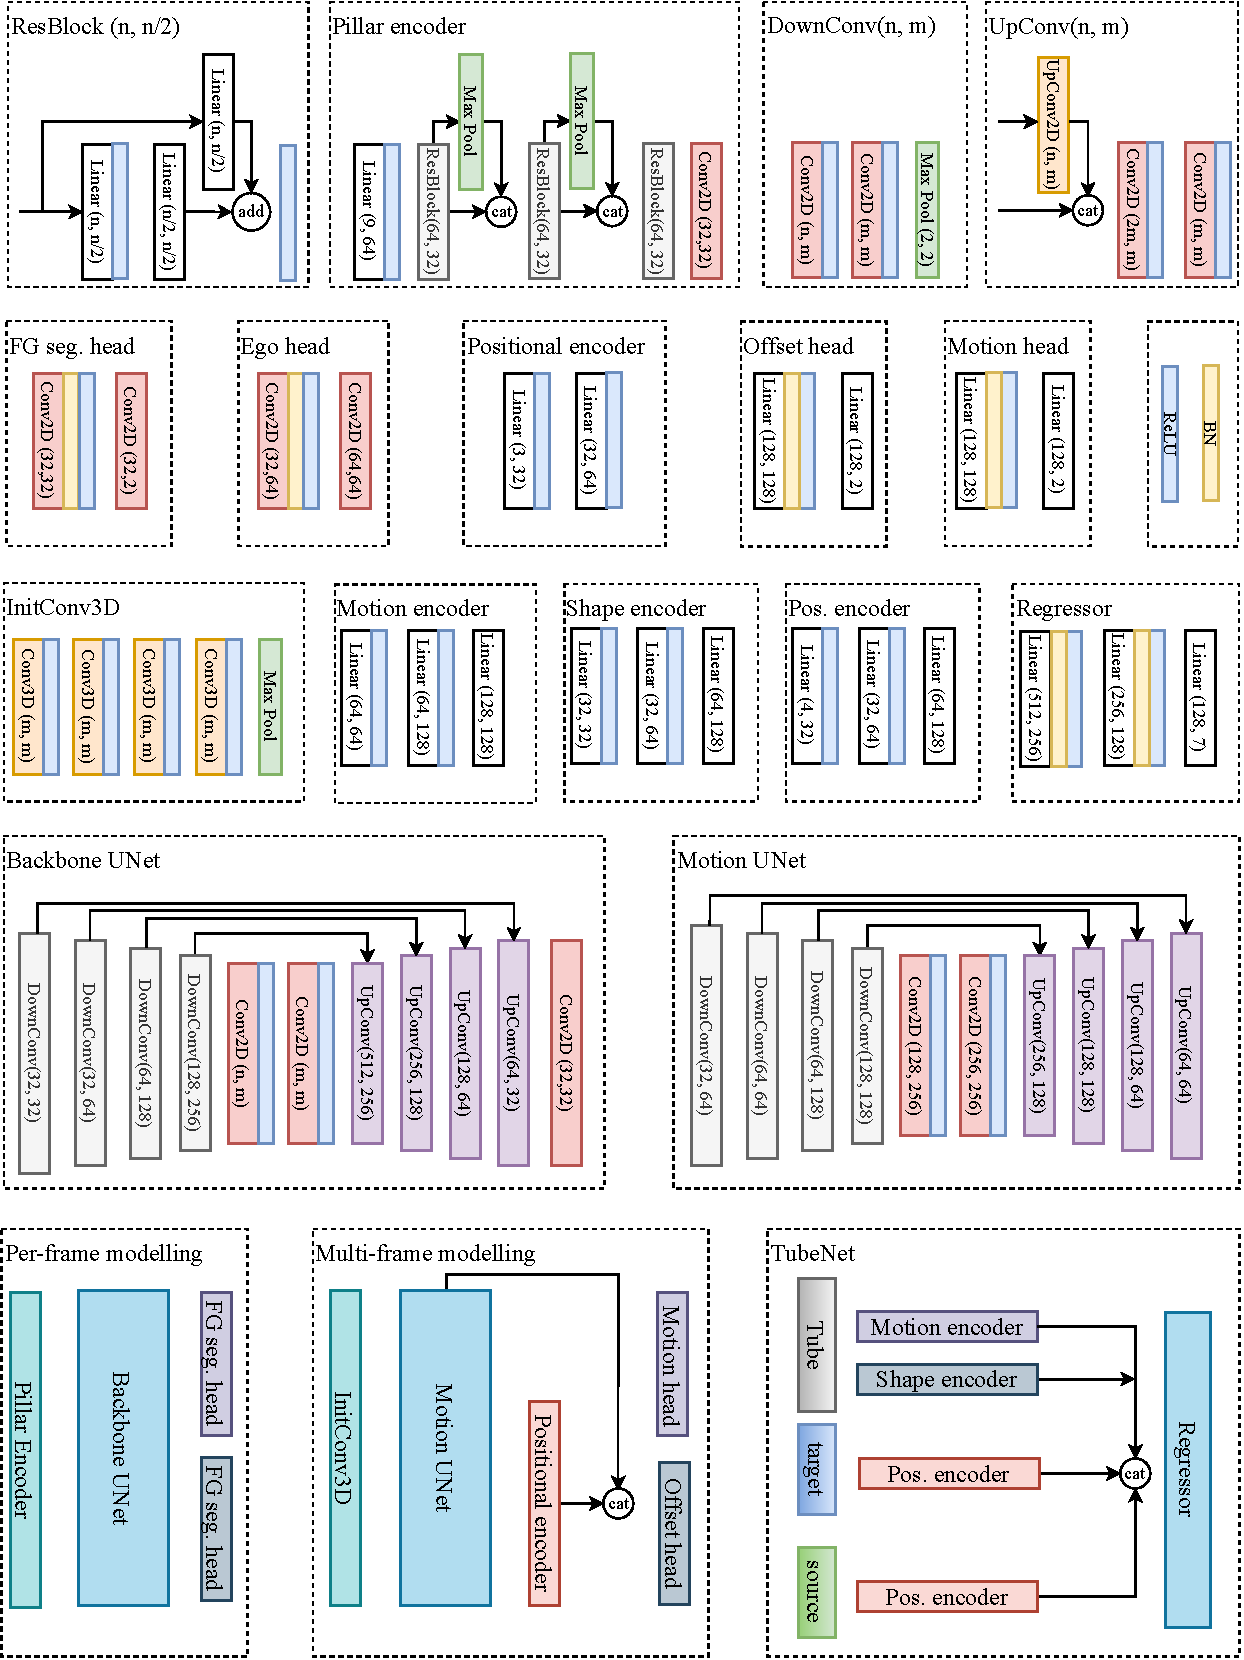
\includegraphics[width=\columnwidth]{figs/figure/network.pdf}
       \caption{Detailed network architecture. All convolutional layers have kernel size 3$\times$3. $(n, m)$ in Conv, UpConv, DownConv, and Linear layers denote the input and output feature dimensions.} 
   \label{fig:supp_network}
\end{figure}